\documentclass{beamer}
%\usetheme{Pittsburgh}
%\usetheme{Rochester}
\usetheme{Madrid}
%\usecolortheme{dolphin}
%\usecolortheme{seahorse}

\usepackage{cmap}				
\usepackage{mathtext} 		
\usepackage[T2A]{fontenc}	
\usepackage[utf8]{inputenc}	
\usepackage[english]{babel}
\usepackage{qtree}
\usepackage{csquotes}
\usepackage[style=apa, sorting=nty, bibencoding=utf8]{biblatex}
\addbibresource{citations.bib}
\DeclareLanguageMapping{british}{british-apa}

\usepackage{hyperref}
\usepackage{graphicx}
\graphicspath{img/}

\title{Blame attribution in autocracies}
\author[]{Vladimir Novikov\\{\small Supervisor: Alexei Zakharov}}
%\centering
\institute[]{National Research University Higher School of Economics}
%\insitute{}
%\logo{
\includegraphics[width = 1cm]{img/logo_с_hse_cmyk_e.png}}
\date{Moscow, 2020}

\begin{document}
%\maketitle

\begin{frame}
    
    \maketitle
    
\end{frame}

\begin{frame}{Blame attribution}
    \begin{enumerate}
    
        
    
        \item Concept of \textbf{blame attribution}: \textbf{public attribution of responsibility} (\textbf{and blame} as the consequence) for government performance;
        
        \item Idea of \textbf{blame avoidance} -- \textbf{blame diffusion}, as a feature of the \textbf{nontransparent system} (not clear who is responsible -- not clear whom to blame), and the basic \textbf{blame shift} and \textbf{responsibility assignment};
        
        \item Examples: Trump blames China for the coronavirus pandemic \parencite{trumpcorona}, Putin assigns this task for the governors \parencite{putincorona}.
        
    \end{enumerate}

\end{frame}


\begin{frame}{The relevance of research}
    \begin{enumerate}
    
        \item \textit{Authoritarian persistence} \parencite{competition}
    
        \item \textit{Third wave of autocratization} \parencite{vdem}
        
        \item \textit{New competitive regimes} \parencite{newway}
        
        \item Most of the authoritarian regimes are the \textit{electoral} ones \parencite{shedler} and due to their past and/or external pressure they hold some democratic features:
        \begin{description}
        
            \item[a)]  These autocracies hold elections (elections can be falsified at some point);
            
            \item[b)] These autocracies \textit{somehow} care about the public opinion \parencite{inform}.
            
        \end{description}
    
    \end{enumerate}
    
\end{frame}

\begin{frame}{The relevance of research}
    \begin{figure}
        \centering
        
        \label{fig1}
        \includegraphics[width=\textwidth,height=0.8\textheight,keepaspectratio]{img/trend2.jpg}
        \caption{1, source: \cite{vdem}}
    \end{figure}
\end{frame}



\begin{frame}{Problem statement}
    %\centering
    
    \begin{enumerate}
    
        \item The puzzle is \textbf{the authoritarian persistence roots} and how \textbf{the logic of blame attribution helps to explain} it;
        
        \item \textbf{Rational choice} and \textbf{formal game theory modelling};
        
        \item The \textbf{subject} of the paper -- \textbf{electoral fraud}, driven by the blame avoidance motivations;
        
        
        \item The question here is \textbf{which strategy would be the optimum} for the actors: self-blame avoidance or survival of the regime at large, and \textbf{how can this optic explain the persistence of authoritarian politics}, i.e. how stable would be the equilibrium?
        
    \end{enumerate}

\end{frame}


\begin{frame}{Problem Statement}
    \centering
    
    I \textbf{aim} to model \textbf{how the blame avoidance and the blame minimizing game} within inner regime actors \textbf{shapes  authoritarian politics}. For these purposes:
    
    \begin{enumerate}
        
        \item Determine theoretical framework;
        
        \item \textbf{I establish a formal model of} statistics and preference falsification, specifically by the example of \textbf{electoral fraud}
        
        \item \textbf{I test the model predictions on two actual cases}
        
    \end{enumerate}
    
\end{frame}

%\begin{frame}{The logic of the game}
    
 %  I study the electoral game in autocracy. For the autocrat it is the way to know the preferences of the people and if his appointed official is good enough. For the official the task is to stay in office by providing potentially falsified election while the people are trying to improve the quality of government by showing their preferences at the election.
    
%\end{frame}


\begin{frame}{\hypertarget{theory}{Existing research and theoretical framework}}
    \begin{enumerate}

        \item Blame attribution is about \textit{whom to blame} for poor performance, if it is unclear who is responsible -- the blame reduces \parencite{econvote_polit, Hood2009};
        
        \item Dictators care about the blame \parencite{autocblame, legislaturesandblame};
        
        \item Autocracies provide elections to gain information \parencite{parties_elections, localfraud};
        
        \item Officials are falsifying the results to seem more competent and loyal \parencite{morethanwin, power_sharing}.
        
    \end{enumerate}
\end{frame}

\begin{frame}{Model setting an logic}
    \centering
    
    There are \textit{two strategic players}: \textbf{the autocrat, the appointed official} \parencite{loyal_competent_1}, and \textbf{the people} -- \textit{a technical player}.
    \\
    \textbf{The autocrat} provides election to get information about the public preferences and to know if his official is good enough.
    \\
    \textbf{The official} want to stay in office, so he can falsify the election and cheat.\\
    The people's \textbf{blame is the difference between the expected and the observed quality} of government.
    
    
    
\end{frame}


\begin{frame}{\hypertarget{time}{The timing of the game}}
    \begin{description}
	    \item[\hyperlink{time1}{$t = 0$}:] {\textbf{The nature} randomly chooses quality of the autocrat and the official;}
	    %And it means also total quality of government and blame $q_t = mean(q_a, q_o), b_{t0} = 1 - mean(q_a, q_o), q_t, b_t  \in [0,1]$;
	    
	    \item[\hyperlink{time2}{$t = 1$}:] { \textbf{The public} observes the total quality of government and \textbf{votes}.\\
	    \textbf{The official} observes the total quality and the people's vote and \textbf{chooses} whether to \textbf{steal the election} or not. After that he reports the final vote;}
	    
	    \item[\hyperlink{time3}{$t = 2$}:] {\textbf{The autocrat's turn}. He observes the reported vote. If the election was lost he can either \textbf{give up power}  or \textbf{call of the election}.\\
	    Regardless of the vote, the autocrat \textbf{chooses if he replaces the official} or not.}
    
	\end{description}
\end{frame}

\begin{frame}{Utilities functions}
    
    \noindent The autocrat is minimizing the blame towards himself and maximizing overall quality of government under condition of staying in power:
	\begin{center}
	    $U_{auto} = \begin{cases}
        q_{total} (1 - blame_{auto}) &  \textbar  \textit{stays in power}\\
        0  & \textbar  \textit{loses power}
	    \end{cases}$
	\end{center}
	
	\noindent The official's goal is to hold his office:
	\begin{center}
	    $U_{off} = \begin{cases}
        1 &  \textbar  \textit{stays in office}\\
        0 &  \textbar  \textit{loses office}
	    \end{cases}$
	\end{center}
	And people are maximizing quality of government: $U_{people} = q_{total}$
    
\end{frame}


\begin{frame}{Results of the baseline model}
    \begin{enumerate}
        
        \item \hypertarget{sum1}{In autocracy} the appointed official can only choose \textit{the portraying loyalty} strategy;
        
        \item The official has incentives to falsify the results to \hyperlink{officialtask}{satisfy two conditions}:
        
        \begin{enumerate}
            \item Elections are won; 
            
            \item The results is \textit{good enough} and his estimated quality is satisfactory.
        \end{enumerate}
        
        \item The game regardless of initial conditions comes for \textbf{the equilibrium where both the autocrat and the official stay in power} (proof at \hyperlink{app1}{the appendix})
        
    \end{enumerate}
\end{frame}


\begin{frame}{\hypertarget{game2}{The game with blame limitation}}
    
    <<Strict>> assumption: excessively high blame leads to revolt:
    
    $$\textit{the autocrat stays in power} =  \begin{cases}
        vote_{reported} > 0.5\\
        blame_{total} < \theta \textbar \theta = 1
	    \end{cases}$$
    
    \hypertarget{prestext2}{Note}, that this restriction does not change the official's strategy (\hyperlink{fig9}{figure 9}) and does not change the autocrat's strategy significantly (proof at the \hyperlink{app2}{appendix}).
    
    
\end{frame}


\begin{frame}{The game with blame limitation: results}
    
    \begin{enumerate}
        
        \item The revolt is possible if both the regime actors are incompetent and fraud was redundant;
        
        \item If at least one of the regime actors is competent the autocrat can reduce the blame by the replacement of the official;
        
        \item Possibility of people's revolt leads to an increase of the expected total quality of government.
        
    \end{enumerate}
    
\end{frame}

\begin{frame}[plain]
    
    \begin{figure}
        \centering
        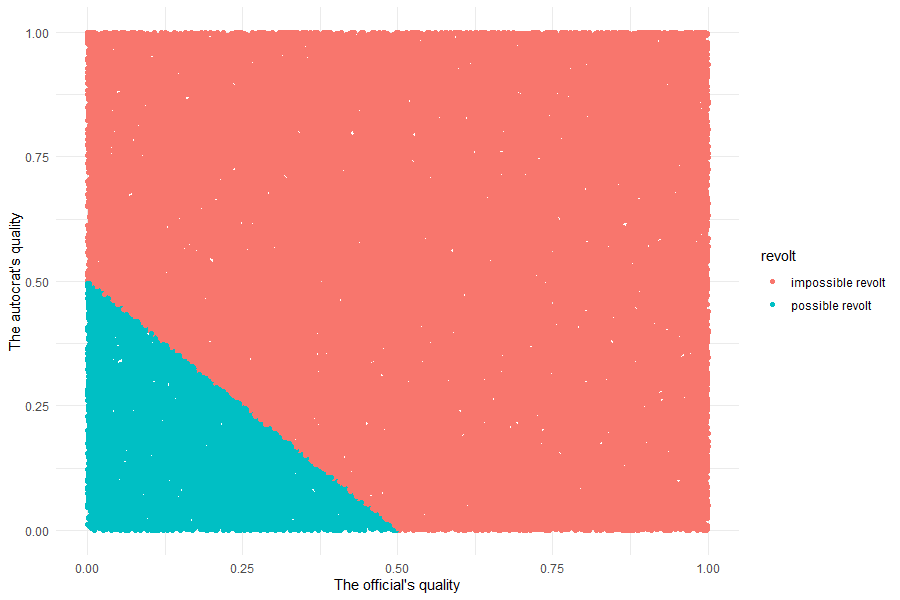
\includegraphics[width=12cm]{img/revolt.png}
        \label{fig9}
    \end{figure}
    
\end{frame}

\begin{frame}{\hypertarget{case1}{Suitability for a case study: the IRP rule in Mexico }}

   Features of the IRP rule taken from \parencite{votingforautocracy}:\\
    \begin{enumerate}
        
        \item The \textbf{IRP regime was supported} more i\textbf{n the underdeveloped regions}%: \textbf{if the region is underdeveloped the expected quality should be lower} and thus\textbf{ the lower is the blame and the higher is the vote};
        
        \item The \textbf{main rivalries for the regime were primary party members}, who have not chosen loyalty.% The official's \textbf{strategies are limited if he depends on the autocrat}, the <<exit option>> would change his behaviour; 
        
        \item \textbf{IRP was forced to give up power not after a massive fraud} in 1988 but after an observed election in 2000.% If there is \textbf{no risk of revolt the fraud is a path to longevity of the regime}.
        
    \end{enumerate}
    
\end{frame}

\begin{frame}{\hypertarget{case2}{Suitability for a case study: contemporary Russian regime}}
    
    \begin{enumerate}
        
        \item \textbf{Dependant lower-level officials allow the consolidation of the regime}. Putin's \textbf{regime consolidated} (\hyperlink{russ}{figure 3}) at the same time \textbf{the direct governors elections were cancelled} \parencite{governors};
        
        \item \textbf{The basic blame avoidance strategy} for the autocrat in case of poor quality of government is \textbf{to replace the official}. \textbf{The central government} in contemporary Russia \textbf{hires governors in any case of poor performance and bad public opinion about the government} \parencite{governors2}.
        
    \end{enumerate}
    
\end{frame}

\begin{frame}[plain]
    \begin{figure}
        \centering
        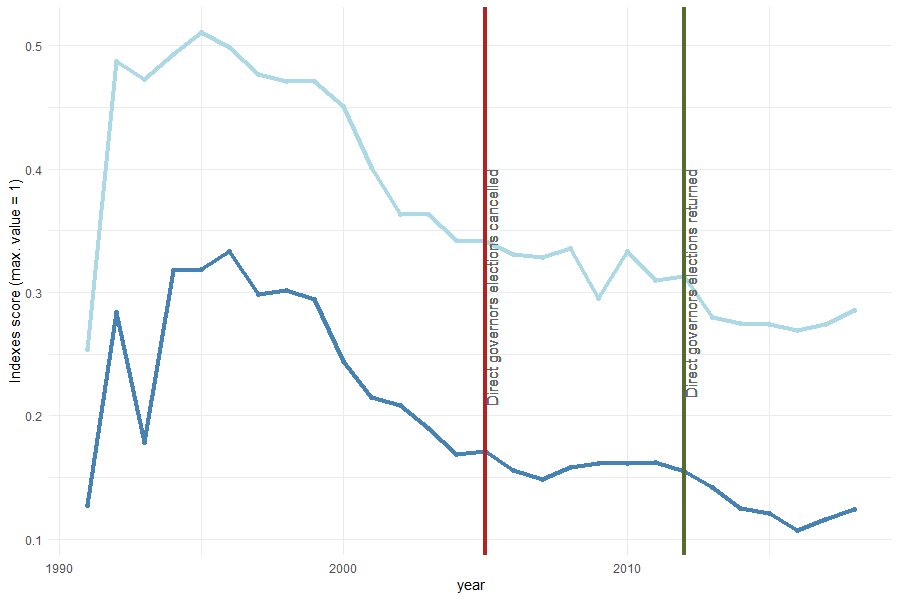
\includegraphics[height=7.5cm]{img/russia_3.png}
        \label{rus}
        \caption{\footnotesize{3 \hypertarget{russ}{Liberal} democracy (dark blue line) and polyarchy (light blue line) indexes scores for Russia, data from the Varieties of Democracy dataset \parencite{vdem_data}}}
    \end{figure}
\end{frame}

\begin{frame}{Outlines for the further development of the models}
    
    \begin{enumerate}
    
        \item Preassigned blame distribution between the autocrat and the official;
        
        \item Media bias which affect the blame distribution;
        
        \item Loyalty-competence dilemma;
        
        \item Government can affect the expected (by the people) quality of government (and thus affect the blame);
        
        \item Further empirical tests are necessary. 
        
    \end{enumerate}
    
    
\end{frame}

\begin{frame}{\hypertarget{concl}{Conclusion}}
    \begin{enumerate}

        
        \item The baseline model can be applied for various statistics falsifications, the game brings the equilibrium with \textbf{all the upcoming information falsified enough} and the regime stays stable;
        
        \item If the \textbf{revolt is possible} and both the autocrat and the official are incompetent the \textbf{expected quality of government increases};
        
        \item However, \textbf{the revolt is still not likely}. That explains \textbf{the stability of the electoral autocracies }under a certain leader, who changes the appointed officials.
        

    \end{enumerate}
    
\end{frame}

\begin{frame}
\huge{\centerline{The End}}
\centerline{Thanks for your attention!}
\end{frame}

\begin{frame}{Appendix: the official's task}
    
     \hypertarget{prestext}{Based} on \hyperlink{fig4}{figure 5} the only way for the official to stay in office is two satisfy \hypertarget{officialtask}{the two following conditions:}
    \begin{enumerate}
        \item $vote_{reported} > 0.5 \Leftrightarrow fraud > 0.5 - vote_{people}$
        
        \item $\hat q_o > 0.5 \Leftrightarrow fraud > \dfrac{0.5 - q_o}{2}, vote_{reported} > q_a + 0.25$
        
    \end{enumerate}

    \noindent Which means:
    $$fraud = max(0.5 - \dfrac{q_a+q_o}{2} + \gamma; \dfrac{0.5 - q_o}{2} +\gamma) \textbar \gamma > 0$$
    
    \noindent The official is able to satisfy these condition for all given qualities (proof in the \hyperlink{app1}{appendix}), \hyperlink{sum1}{back to text.}
    
\end{frame}

\begin{frame}{\hypertarget{app1}{Appendix 1: proof for the baseline model}}

    Taking $q_a, q_o = \alpha, \omega \in [0,1]$\\
    Thus $q_t = \dfrac{\alpha+\omega}{2}, blame_t = 1 - \dfrac{\alpha+\omega}{2}, vote_t = \dfrac{\alpha+\omega}{2}$\\
    Based on \hyperlink{fig4}{figure 5} the official's task:    $$fraud = max(0.5 - \dfrac{\alpha+\omega}{2} + \gamma; \dfrac{0.5 - \omega}{2} +\gamma) \textbar \gamma > 0$$
    $$vote_{reported} = \dfrac{\alpha+\omega}{2} + max(0.5 - \dfrac{\alpha+\omega}{2} + \gamma; \dfrac{0.5 - \omega}{2} + \gamma)$$
    $$vote_{reported} \geq \dfrac{\alpha+\omega}{2} + 0.5 - \dfrac{\alpha+\omega}{2} + \gamma = 0.5 + \gamma > 0.5$$ 
    $$vote_{reported} \geq \dfrac{\alpha+\omega}{2} + \dfrac{0.5 - \omega}{2} +\gamma = \dfrac{\alpha + 0.5}{2} + \gamma$$
    $$\hat q_o = 2 vote_{reported} - \alpha = \alpha + 0.5 + 2\gamma - \alpha = 0.5 + 2\gamma > 0.5$$
    \textbf{So both conditions are satisfied} $\forall \alpha, \omega \in [0,1]$; \hyperlink{prestext}{back to text}.
    
    

\end{frame}


\begin{frame}{\hypertarget{app2}{Appendix 2: proof for the model with blame restriction}}
    The equilibrium outcome's total amount of blame:\\ $b_{t} = 1 - q_t + fraud$, $blame_{total} < \theta = 1$\\
    $max(0.5 - \dfrac{\alpha+\omega}{2} + \gamma; \dfrac{0.5 - \omega}{2} +\gamma)= \begin{cases}
        0.5 - \dfrac{\alpha+\omega}{2} + \gamma & \textbar \alpha \leq 0.5 \\ 
        \dfrac{0.5 - \omega}{2} +\gamma & \textbar \alpha > 0.5
    \end{cases}$\\
    So for $\alpha \leq 0.5$:\\
    $\begin{cases}
    b_t \geq \theta = 1 & \textbar  \dfrac{\alpha+\omega}{2} = q_t \leq 0.25 \Leftrightarrow \omega \leq 0.5\\
    b_t < \theta = 1 & \textbar  \dfrac{\alpha+\omega}{2} = q_t > 0.25
    \end{cases}$\\
    For $\alpha \geq 0.5$:\\
    $\begin{cases}
        b_t \geq 1 & \textbar \omega = 0\\
        b_t < 1 & \textbar \omega > 0
    \end{cases}$
    \\\hyperlink{prestext2}{back to text}
\end{frame}

\begin{frame}{\hypertarget{time1}{Appendix: The timing of the game}}
    \begin{description}
	    \item[$t = 0$:] {\textbf{The nature} randomly chooses quality of the autocrat and the official: $q_a, q_o$ uniformly distributed $\in [0,1];$, which are independent variables}
    \end{description}
    \hyperlink{time}{back}
\end{frame}

\begin{frame}{\hypertarget{time2}{Appendix: The timing of the game}}
    \begin{description}
	    \item[$t = 1$:] { \textbf{The public} observes the total quality of government $q_t = (q_a +q_o) /2$ and \textbf{votes}, the people's vote if the function from blame $v_p = 1-blame_t$. Whereas $blame_t = E(q_t) - q_t$ $\textbar E(q_t) = 1$; the people's vote $vote_p$ is known by the people and observed by the official, but not by the autocrat.\\
	    \textbf{The official} observes $q_t$ and $vote_p$ and \textbf{chooses} whether to \textbf{steal the election} or not: if the election was stolen $vote_r = vote_p + fraud$, $vote_r$ is published and becomes a public information;\\
	    $fraud \in [0,1]$ is basically the share of votes that were stolen;}
    \end{description}
    \hyperlink{time}{back}
\end{frame}

\begin{frame}{\hypertarget{time3}{Appendix: The timing of the game}}
    \begin{description}
    \item[$t = 2$:] {\textbf{The autocrat's turn}. He observes $v_f$. If the election was lost $vote_{reported} < 0.5$ the autocrat can either \textbf{give up power} which will end the game or \textbf{annul election results}, thereby addressing the blame towards the autocrat himself.\\
	    Regardless of the vote, the autocrat \textbf{chooses if he replaces the official} or not. If the official was removed the blame declines, so $\Delta blame_t, \Delta blame_a < 0$.}	   
	\end{description}
	\hyperlink{time}{back}
\end{frame}


\begin{frame}{Appendix: the official's turn}
    
    \begin{figure}
        \centering
        
        \Tree[.\textbf{The people vote: }$Vote_{p}=q_{t}$\\\textbf{The official's turn:} [.\textbf{Chooses fraud?} [.Yes $vote_{reported}=Vote_{p}+Fraud>0.5$\\$\Delta Blame_{total}=Fraud$ ]
                [.No $vote_{reported}=Vote_{people}$\\$\Delta Blame_{total}=0$ ]]]
        \caption{4: the official's game tree}
        \label{fig3}
        
    \end{figure}
    
\end{frame}

\begin{frame}{Appendix: the official's turn}
    
    \begin{figure}
        \centering
       \footnotesize{
        \Tree[.\textbf{The official reports the final vote} [.$vote_r>0.5$\\\textbf{The autocrat estimates the official's quality:}\\$\hat q_o=2vote_{r}-q_a\Leftrightarrow vote_{r}>\frac{0.5-q_o}{2}$ [.$\hat q_o\geq0.5=E(q_o)$ [.\textbf{The official stays}\\\textit{Estimated quality better}\\\textit{than expected} ]]
               [.$\hat q_o<0.5=E(q_o)$ [.\textbf{The official replaced}\\\textit{Estimated quality worse}\\\textit{than expected} ]]]
          [.$vote_r\leq0.5$ [.\textbf{The official anyway is replaced:}\\\textit{by the autocrat (to shift blame)}\\\textit{or due to regime change} ]]]}
        \label{fig4}
         \caption{5 \hypertarget{fig4}{the official's game tree with outcomes}; \hyperlink{prestext}{back to text}}
        
    \end{figure}
    
    
    
    
    
\end{frame}

\begin{frame}{Appendix: the autocrat's turn}
    
    \begin{figure}
        \centering
       \footnotesize{
        \Tree[.\textbf{The official reports the final vote: }$vote_{reported}>0.5$\\\textbf{The autocrat estimates the official quality:} [.$\hat q_o\geq0.5=E(q_o)$ [.\textit{The official stays}\\\textit{The autocrat stays}\\\textit{The blame is constant} ]]
               [.$\hat q_o<0.5=E(q_o)$ [.\textit{The autocrat replaces}\\\textit{the official:}\\\textit{as $\hat q_o < E(q_o)$} [.\textit{The autocrat stays}\\\textit{The official replaced}\\\textit{The blame is reduced} ]]]
    ]
        
        
        }
        \label{fig5}
         \caption{6 the autocrat's game tree if the election was won}
        
    \end{figure}
    
\end{frame}

\begin{frame}{Appendix: the autocrat's turn}
    
    \begin{figure}
        \centering
       \footnotesize{
        
        \Tree[.\textbf{The official reports the final vote: }$vote_{reported}\leq0.5$\\\textbf{The autocrat calls off the election?} [.No [.\textit{The regime gives up power:}\\\textit{Both the official and}\\\textit{the autocrat replaced} ]]
               [.Yes [.\textbf{The autocrat replaces the official?} [.Yes\\\textit{The blame is reduced} ] [.No\\\textit{The blame is constant} ] ] ]]
        
        }
        \label{fig6}
         \caption{7 the autocrat's game tree if the election was lost}
        
    \end{figure}
    
\end{frame}

\begin{frame}{Appendix: the autocrat's turn}
    
    \begin{figure}
        \centering
       
       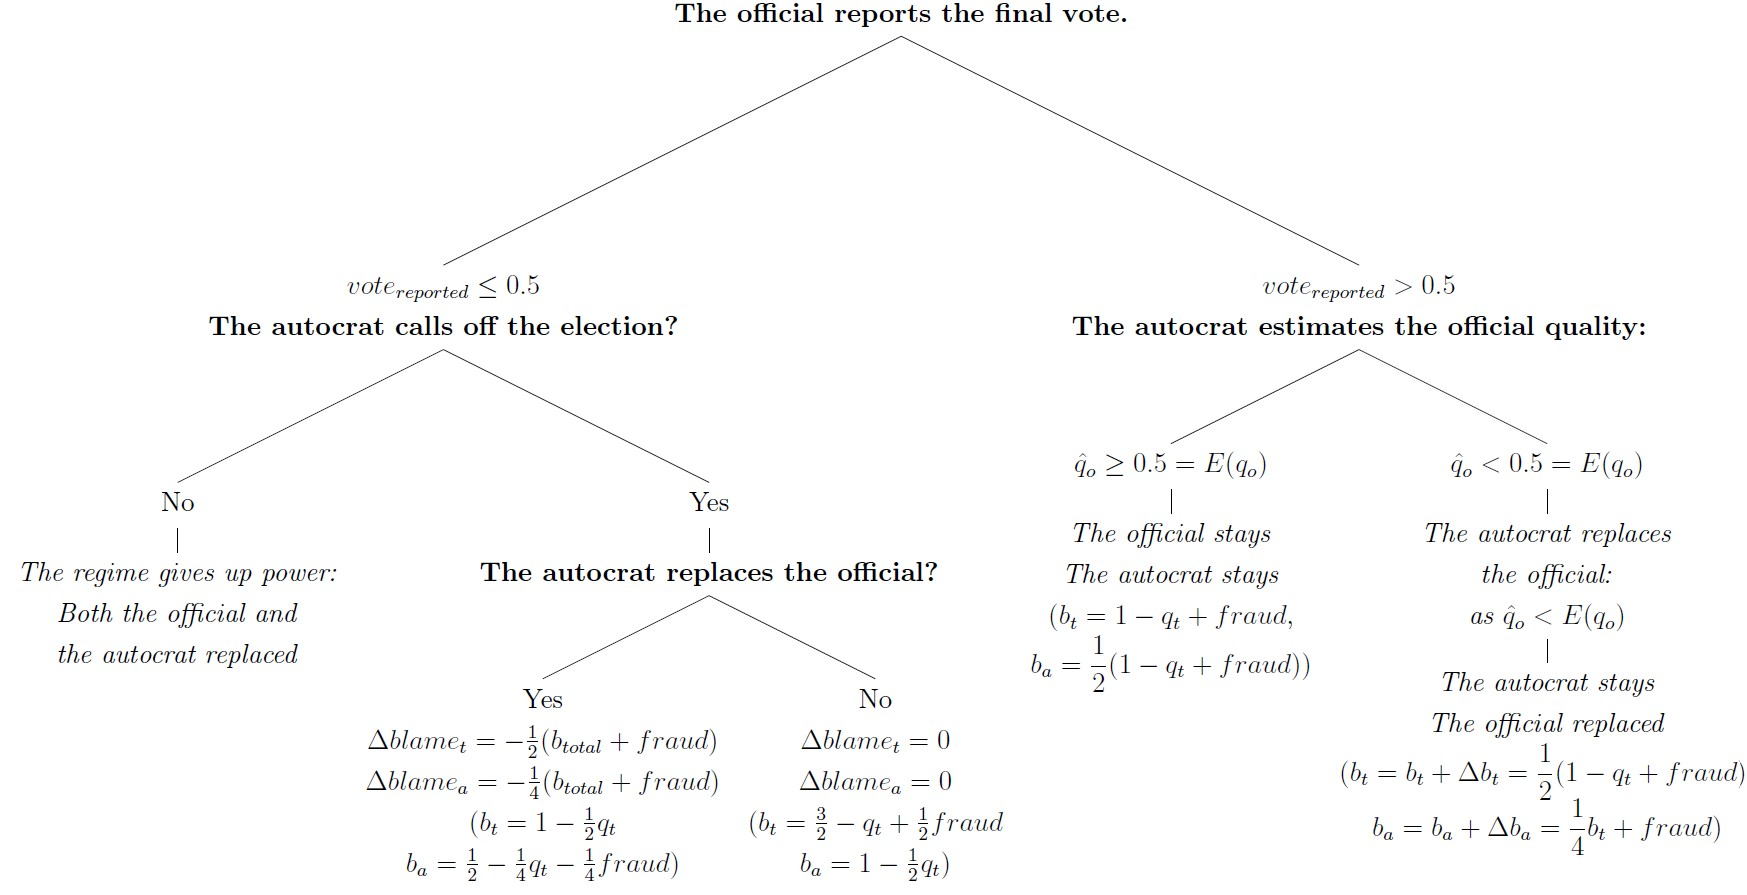
\includegraphics[width=\textwidth]{img/autocratgametree.jpg}
       
        \label{fig7}
         \caption{8 full the autocrat's game tree}
        
    \end{figure}
    
\end{frame}


\begin{frame}{Appendix: the official's turn}
    
    \begin{figure}
        \centering
       \footnotesize{
       
       \Tree[.\textbf{The official reports the final vote} [.$vote_r>0.5$\\\textbf{Estimated quality $q_o$ satisfactory?}\\$\hat q_o=2vote_{r}-q_a$ [.Yes\\$\hat q_o\geq0.5=E(q_o)$\\\textbf{$b_{total}$ exceeds threshold?} No,$b_t<\theta$\\\textbf{Stays} Yes,$b_t\geq\theta$\\\textbf{Replaced}     ]
               [.No\\$\hat q_o<0.5=E(q_o)$ [.\textbf{Replaced} ]]]
          [.$vote_r\leq0.5$ [.\textbf{Replaced} ]]]
       
       }
        \label{fig8}
         \caption{9 \hypertarget{fig8}{the official's game tree with outcomes} }
        
    \end{figure}
    
\end{frame}

\end{document}
